\chapter{Cloud Architecture Design Patterns}

This chapter introduces different design patterns that were used in Chapter \ref{chap:ad}. It aims to provide some background on the chosen patterns and justify their requirement. A short description of how these patterns are applied in the prototype \index{Prototype} is also provided as well as relevant technologies used in conjunction.

\section{Cloud Design Patterns \& Multi-tenancy}
\index{Multi-tenant}

A fundamental decision in any software and system architecture venture is choosing appropriate design patterns. Wilder \cite{Wilder2012-so} defines design patterns as an approach that can be duplicated in order to produce an exact and expected outcome. One of the most referenced definitions of a pattern is by Alexander et. al which states that a pattern describes a problem that occurs over and over in our environment, and then describes the core of the solution to that problem in such a way that you can use the solution a million times over, without ever doing it the same way twice \cite{Alexander1977-ni}. In order to address some of the requirements of the system and help solve some problems that are introduced by using a multi-tenant approach, implementation of some design patterns are necessary. Some of these problems include addressing scalability, handling server load spikes and variations and tenant isolation. 

\textit{Note: The selection of these patterns are a result of an modified Attribute-Driven Design Approach (see section \ref{sec:add}) and qualitative interpretation of its results (see section \ref{sec:arcdrivers}).}

\section{Eventual Consistency}

Brewer's cap theorem, although a common misnomer \cite{Brewer2012}, is often used to justify the implementation of eventual consistency using NoSQL over traditional Relational Database Management Systems (RDBMS ) \cite{Wilder2012-so}. Distributed cloud systems have embraced the idea of eventual consistency as preventing downtime is of higher importance than providing consistent data. In many applications, it is acceptable to serve somewhat stale data as long as the application continues to run even in cases of node failures. The concept of eventual consistency states that although the system attempts to be consistent, there is a short tolerated delay in consistency which exists while data updates gets propagated \cite{Wilder2012-so}. Since it is important for our system to remain online and working even in the case of node failure and at the cost of consistency an approach that favours availability has been taken in the choosing of design patterns to apply. The system will also attempt to adhere to the Basically Available, Soft State and Eventually Consistent (BASE) guarantees over the Atomicity, Consistency, Isolation and Durability (ACID) guarantees.
 
 
\section{Command Query Responsibility Segregation (CQRS)}
\index{Command Query Responsibility Segregation (CQRS)}
 
CQRS is a popular design pattern used in scalable cloud based applications. At its core, the pattern is defined as a separation between the queries (data requests) operations and commands (data modification) \cite{Homer2014}. This stands in contrast to traditional CRUD operations that are all handled together using the same model or entity. The argument for separating these operations includes reduced complexity of domain models, increased scalability and simplification of implementation \cite{Homer2014}. Scalability is improved by allowing read and write stores scaled independently depending on usage. Implementation is simplified and performance is improved since views can be composed according to View Models and data can be de-normalized in order to improve queries. Although the pattern does not implicitly require the separation of data stores, it is useful to consider for building cloud -native applications. 
 
CQRS embraces the fact that consistency of data is given up in order to provide better availability \index{Availability} and partitioning and therefore does not try to solve the problems of stale data. Instead, it explicitly understands that data is stale and would be updated to be eventually consistent. The CQRS pattern is commonly used in conjunction with Event Sourcing in order to construct a write only stream of commands that are executed in order to modify the data \cite{Homer2014}. However due to the complexities involved with setting up a complete event subscriber/publisher workflow around the Event Sourcing pattern a Queue Centric Workflow pattern has been used as alternative. Another advantage of CQRS is it significantly simplifies the need for transformations of models between layers since the query operations could select related view data directly into View Models without needing to transpose the other layers. In its essence, CQRS works with the fact that if you try to optimize a single domain object for both commands and queries, it would become bloated and ineffective at either. In the system we attempt to implement CQRS (Without Domain Driven Design (DDD)) by clearly separating the workflow of our commands and queries, including separation of models all the way through to repositories. Figure \ref{fig:CQRS} shows the high level breakdown of application layers and query vs. command workflow. One of the major obstacles in implementing CQRS however is the fact that since commands are processed independently from queries, commands cannot return the modified object \cite{Homer2014}. This means that users should be notified that their command has been queued for execution but they cannot be guaranteed to see the results immediately. Instead alternative mechanisms might be considered in order to notify users that their commands have been processed such as SignalR push technologies. This is also an extremely important fact to mind during UI design.
 
 
\section{Queue Centric Workflow}
\label{sec:qcw}
\index{Queue Centric Workflow}
 Queue Centric Workflow (QCW) patterns describe a method for loosely coupling requests between the presentation layer and lower application layers as seen in figure \ref{fig:CQRS}. A common problem with SaaS \index{Software as a Service (SaaS)} implementations is its unpredictable loads \cite{Homer2014}. In multi-tenant applications this becomes an even bigger issue as spikes in usage from one tenant directly impact other tenants \cite{Betts2012-ad}. In order to isolate tenants from the impacts of load spikes a QCW based load levelling pattern has been implemented. The pattern describes the introduction of a queue between tasks and services that run asynchronously \cite{Wilder2012-so}. A task posts a message into a queue that contains all required data relevant to its execution. A service then retrieves these messages and processes them at a consistent rate. This allows the queue to act as a buffer protecting the service from becoming flooded and affected to dramatically by load spikes.
It is also possible to scale the service that processes queue messages in order to handle increased queue loads. In our project we considered using an Azure Worker Role \ref{appendix} to be setup as a service that consumes our queued tasks and executes them. However, due to the lower costs and ease of implementing Azure WebJobs compared to worker roles this option was used for demonstration purposes instead. Migration between these two Azure services is extremely simple and required minimal modification if it would be required for production implementation. The prototype uses the CQRS workflow as seen in figure \ref{fig:CQRSFlow}. A Console Application that is hosted as WebJob runs continuously and consumes messages from Azure Storage Queues \ref{appendix}. The presentation layer creates tasks in the form of commands (see below) that is posted to the queue and then executed in a consistent manner by the WebJob.
 
\begin{figure}
\centering
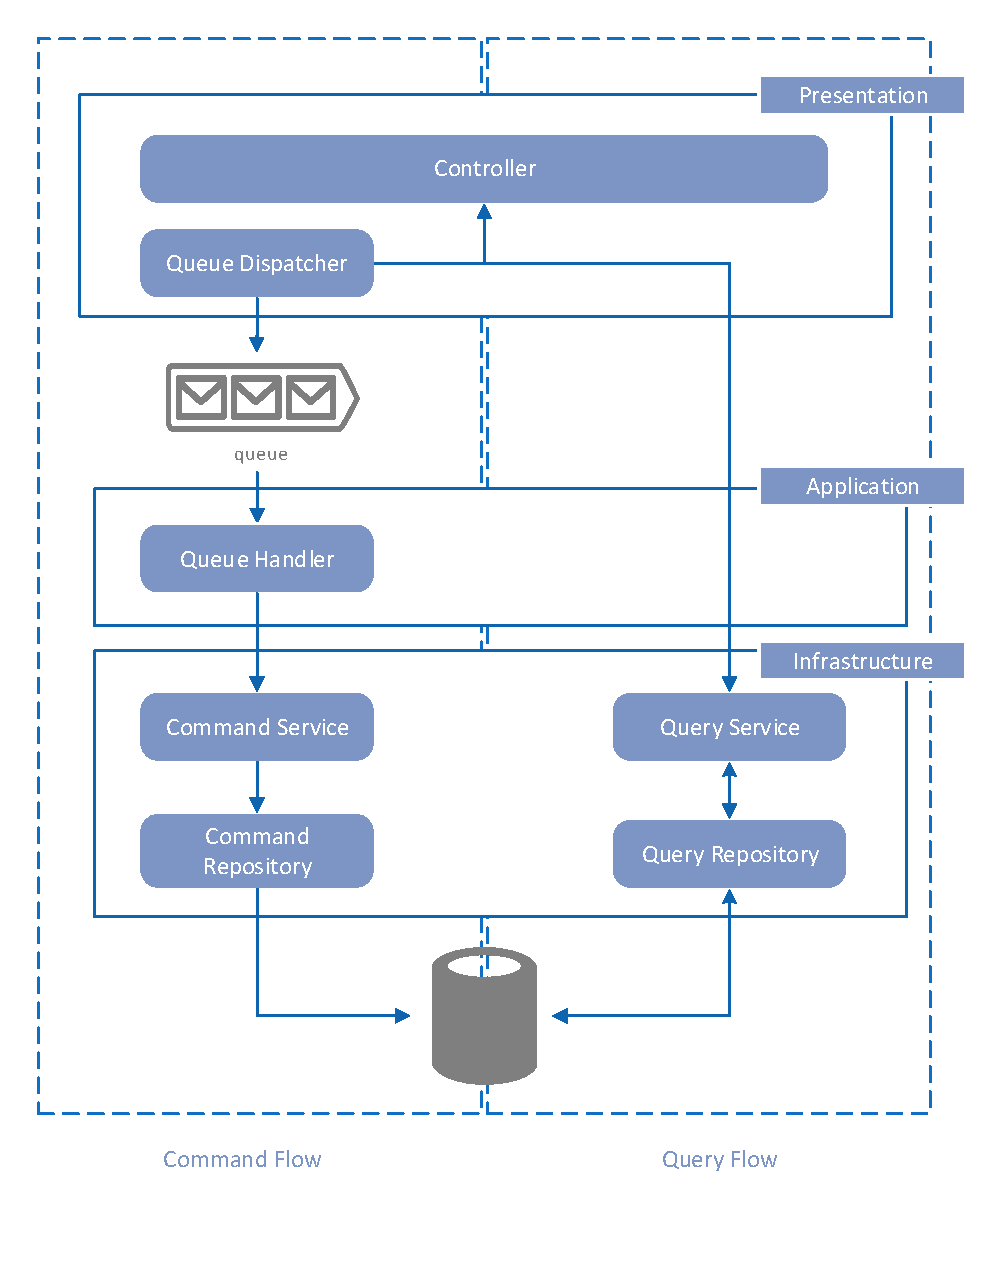
\includegraphics[width=\textwidth]{CQRSFlow}
\caption{CQRS, QCW and Command pattern work flow}
\index{Command pattern}
\label{fig:CQRSFlow}
\end{figure}
 
 
 \section{Command Pattern}
 
 The command pattern uses a uniform interface that isolates execution data from the invoker. This is achieved by exposing only an execute method that when called handles delegation of the requests implementation to other objects \cite{Gamma1994-ho}. The command pattern is useful when combined with other patterns such as CQRS, Event Sourcing and especially with QCW patterns. The command pattern also allows us to create specific command objects that represent real world business cases and helps move more to DDD. Command objects are also useful as they encapsulate all the information required for delayed execution \cite{Gamma1994-ho} as is central to queue or message based implementations. In our prototype the command pattern is used to encapsulate all modifications to data in our data stores. The controllers create command objects and then pass these into a queue via our queue service. A worker role/WebJob that constantly queries the queue then picks up these commands and invoke their execute command. This way our presentation layer never executes any commands and contains no references to our command repositories or services. It simply uses the queue service to line up commands for execution. This separation of command implementation from command invocation can help us create a highly scalable system based on eventual consistency.
 
 
 \section{Cache Aside Pattern}
  \label{sec:cache}
 Application performance can significantly be improved by implementing a caching solution. By using a cache an application reduces the amount of calls to its data stores and instead reads commonly used data from a cache. Instead of using persistent storage to hold data, caches are usually implemented in memory and these significantly increase its read and write speeds. However, caches data need to be constantly maintained in order to ensure consistency. One pattern that helps with solving the consistency issue between the data store and the cache is the Cache Aside pattern. This is a very simple pattern that describes using three basic steps in order to ensure cache data is updated \cite{Homer2014}:
 
    \begin{enumerate}
        \item On query request, check if the item is currently in the cache
        \item If the item is in the cache it returns the cached version
        \item If the item is not in the cache, retrieve it from storage and save it to the cache
   \end{enumerate}
   
 
On command requests the object in the cache should be invalidated in order to be retrieved again on its next query request. For this thesis the Cache Aside pattern is used in combination with Azure Redis Cache.\index{Azure!Azure Redis Cache} The cache is updates are handled in the service layer. Any queries retrieve the data from its respective storage and then serialized and added to the cache. Any commands delete the cache item with a cache key corresponding to the id.


\section{Conclusion}
 
Multi-tenant applications introduce specific problems that are solvable through application of design patterns. Firstly the problem of tenant isolation is addressed through application of a QCW pattern or more precisely, a queue based load levelling pattern. This QCW pattern is further extended by applying the command pattern, effectively turning tasks into self containing objects that could be queued up for later execution. The problem of scalability is also addressed by implementing the QCW as it allows commands to be lined up and handled in the asynchronously and in the background. This alone however is not enough to be considered truly cloud -native and scalable. In order to ensure easy scalability, the CQRS pattern is introduced. This pattern helps to separate all query operations from command operations all the way down to the models.
 
This combined with the QCW allows the application to easily scale its command processing by provisioning more instances of the queue handler. Similarly, it also provides the ability for the query processing through provisioning of more read only data stores to be accessed. These patterns are used in conjunction with the Cache Aside pattern through storing data in the cache on query operations and deleting items from the cache on command operations provides improved overall performance. Instead of attempting to ensure consistency in the system, availability is considered higher priority and thus allows the implementation of these patterns in ensuring the BASE guarantees are met.